
\chapter*{Dev Notes}

\section{Concretizing less does not infer spuriousness}

\subsection{Concrete AF}

\begin{center}
	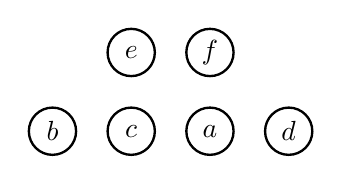
\begin{tikzpicture}
		\def \ax{2.0} \def \ay{-1.0}
		\def \bx{0.0} \def \by{-1.0}
		\def \cx{1.0} \def \cy{-1.0}
		\def \dx{3.0} \def \dy{-1.0}
		\def \ex{1.0} \def \ey{0}
		\def \fx{2.0} \def \fy{0}
  
        % Singletons
        \draw[line width=0.3mm] (\ax,\ay)  circle (0.3) node[anchor=center]{$a$};
        \draw[line width=0.3mm] (\bx,\by)  circle (0.3) node[anchor=center]{$b$};
        \draw[line width=0.3mm] (\cx,\cy)  circle (0.3) node[anchor=center]{$c$};
        \draw[line width=0.3mm] (\dx,\dy)  circle (0.3) node[anchor=center]{$d$};
        \draw[line width=0.3mm] (\ex,\ey)  circle (0.3) node[anchor=center]{$e$};
        \draw[line width=0.3mm] (\fx,\fy)  circle (0.3) node[anchor=center]{$f$};
		% Attacks
		\DrawAttackHorizontal{L}{\cx}{\cy+0.08}{\bx}{\by+0.08}
		\DrawAttackHorizontal{R}{\bx}{\by-0.08}{\cx}{\cy-0.08}
		\DrawAttackHorizontal{R}{\cx}{\cy}{\ax}{\ay}
		\DrawAttackHorizontal{R}{\ax}{\ay}{\dx}{\dy}
		\DrawAttackHorizontal{R}{\ex}{\ey}{\fx}{\fy}
		\DrawSelfAttackLeftTopCluster{\ex-0.1}{\ey + 0.3}
        
		\DrawAttackDiagonal{PLR}{\bx}{\by}{\ex}{\ey}
        \DrawAttackVertical{D}{\fx}{\fy}{\ax}{\ay}
	\end{tikzpicture}
\end{center}
\textbf{Stable Sets:} $\{ b, d, f\}$

\subsection{Abstract AF}
\begin{center}
	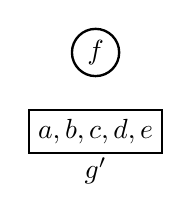
\begin{tikzpicture}
		\def \fx{1.0} \def \fy{ 0.0}
		\def \gx{1.0} \def \gy{-1.0}
        % Clusters
        \node[rectangle, draw, line width=0.3mm] at (\gx, \gy) {$a,b,c,d,e$};
		\node at (1, -1.5) {$g'$};
        % Singletons
        \draw[line width=0.3mm] (\fx,\fy)  circle (0.3) node[anchor=center]{$f$};
		% Attacks
		\DrawAttackVertical{B}{\fx}{\fy}{\gx}{\gy}
		\DrawSelfAttackLeftTopCluster{\gx-0.8}{\gy + 0.3}
	\end{tikzpicture}
\end{center}
\textbf{Stable Sets:} $\{ g'\}$, $\{ f, g'\}$, $\{ f\}$

Abstract AF is \textbf{spurious} to concrete AF because sets $\{ g'\}$ and $\{ f\}$.



\subsection{Concretized AF (a,b,d,e)}
\begin{center}
	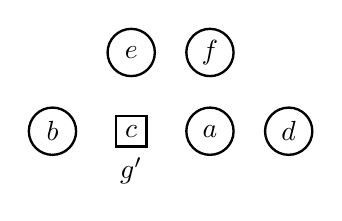
\begin{tikzpicture}
		\def \ax{2.0} \def \ay{-1.0}
		\def \bx{0.0} \def \by{-1.0}
		\def \gx{1.0} \def \gy{-1.0}
		\def \dx{3.0} \def \dy{-1.0}
		\def \ex{1.0} \def \ey{0}
		\def \fx{2.0} \def \fy{0}
        % Clusters
        \node[rectangle, draw, line width=0.3mm] at (\gx, \gy) {$c$};
		\node at (1, -1.5) {$g'$};
        % Singletons
        \draw[line width=0.3mm] (\ax,\ay)  circle (0.3) node[anchor=center]{$a$};
        \draw[line width=0.3mm] (\bx,\by)  circle (0.3) node[anchor=center]{$b$};
        \draw[line width=0.3mm] (\dx,\dy)  circle (0.3) node[anchor=center]{$d$};
        \draw[line width=0.3mm] (\ex,\ey)  circle (0.3) node[anchor=center]{$e$};
        \draw[line width=0.3mm] (\fx,\fy)  circle (0.3) node[anchor=center]{$f$};
		% Attacks
		\DrawAttackHorizontal{L}{\gx+0.1}{\gy+0.08}{\bx}{\by+0.08}
		\DrawAttackHorizontal{R}{\bx}{\by-0.08}{\gx+0.1}{\gy-0.08}
		\DrawAttackHorizontal{R}{\gx-0.1}{\gy}{\ax}{\ay}
		\DrawAttackHorizontal{R}{\ax}{\ay}{\dx}{\dy}
		\DrawAttackHorizontal{R}{\ex}{\ey}{\fx}{\fy}
		\DrawSelfAttackLeftTopCluster{\ex-0.1}{\ey + 0.3}
        
		\DrawAttackDiagonal{PLR}{\bx}{\by}{\ex}{\ey}
        \DrawAttackVertical{D}{\fx}{\fy}{\ax}{\ay}
	\end{tikzpicture}
\end{center}
\textbf{Stable Sets:} $\{ b, d, f\}$, $\{ b, d, f, g'\}$

Concretized AF (a,c,d,e) is \textbf{spurious} to concrete AF because set $\{ b, d, f, g'\}$.


\subsection{Concretized AF (e)}
\begin{center}
	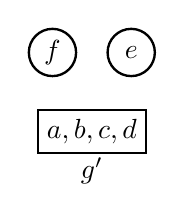
\begin{tikzpicture}
		\def \fx{0.5} \def \fy{ 0.0}
		\def \ex{1.5} \def \ey{ 0.0}
		\def \gx{1.0} \def \gy{-1.0}
        % Clusters
        \node[rectangle, draw, line width=0.3mm] at (\gx, \gy) {$a,b,c,d$};
		\node at (1, -1.5) {$g'$};
        % Singletons
        \draw[line width=0.3mm] (\fx,\fy)  circle (0.3) node[anchor=center]{$f$};
        \draw[line width=0.3mm] (\ex,\ey)  circle (0.3) node[anchor=center]{$e$};
		% Attacks
		\DrawAttackVertical{D}{\fx}{\fy}{\gx-0.5}{\gy}
		\DrawAttackVertical{U}{\gx+0.5}{\gy}{\ex}{\ey}
        \DrawAttackHorizontal{L}{\ex}{\ey}{\fx}{\fy}
		\DrawSelfAttackLeftTopCluster{\gx-0.7}{\gy + 0.3}
		\DrawSelfAttackLeftTopCluster{\ex-0.1}{\ey + 0.3}
	\end{tikzpicture}
\end{center}
\textbf{Stable Sets:} $\{ g', f\}$

Concretized AF (e) is \textbf{faithful} to concrete AF.


